\RequirePackage[T1]{fontenc}
\documentclass[conference,10pt]{IEEEtran}
\usepackage{amsmath,amssymb,graphicx,url}
\title{Current-STA Transactional Repair for Timing--Resource Tradeoffs in 3D FPGA Routing}
\author{\IEEEauthorblockN{Anonymous development manuscript}}
\begin{document}
\maketitle
\begin{abstract}
Legal FPGA routes trade timing, wire and vertical resources. Our current-STA repair searches connection groups on private trees and commits after physical, capacity and native timing checks. Retained-crossing domains encourage sharing; search failure releases the affected network's domain. Three timing repairs improve strong native BNN from 13.607436 to 13.228146 ns for forty extra wire units. From identical fresh roots, native/domain-first flows take 7933.25/9754.31 s at equal final CPD; domain-first spends 1786 wire for 39 fewer SB/two fewer CB, attaining a fixed-terminal vertical bound. Matched owner-scope repairs escape a certified single-net local minimum with unchanged endpoint vectors. Independent feedback improves ten setup components without regressions. Fixed-input controls expose grouping, timing-budget and acceptance-scheduling tradeoffs. Robot transfer saves one CB for 20 wire; both conv-layer roles fail initial routing. Single-pass indexing preserves BNN execution at 7463.17 s. Mechanism ablations separate sharing domains, failed-search release and owner coordination. Complete frozen-controller confirmation on distinct physical inputs remains pending.
\end{abstract}
\begin{IEEEkeywords}
3D FPGA, detailed routing, static timing analysis, transactional repair, multiobjective optimization
\end{IEEEkeywords}

\section{Problem and Motivation}
Three-dimensional FPGA routing couples directed reachability, scarce vertical channels and timing. With packing, placement and architecture fixed, repair may improve CPD or trade resources under an explicit timing requirement. Shorter local connections need not improve the complete route: another endpoint may become critical or capacity may block another network.

VTR supplies routing and timing infrastructure~\cite{vtr9paper}. Following Escaping Flatland's separation of design tradeoffs~\cite{flatland}, each comparison fixes its physical input. Reduced fixed-device occupancy does not imply silicon-area or power savings.

We use current STA to select groups, search native replacements and validate complete routes: sharing proxies alone omit timing, retained branches and convergence. 


PathFinder resolves resource competition through negotiated congestion and timing-aware search~\cite{pathfinder}; our native search retains that foundation. We address post-route group selection, vertical sharing and transaction acceptance. Escaping Flatland addresses 3D placement~\cite{flatland}; here placement is fixed. VTR supplies the native legality and STA reference~\cite{vtr9paper}. The contribution is a measured timing--resource repair framework and mechanism-specific evidence, rather than a replacement claim for those placement or routing systems.

The evidence supports three concrete contributions: current-state whole-group repair with explicit acceptance and rollback; separation of domain restriction, failure release and owner coordination; and complete-cost comparisons retaining infeasible inputs and unfavorable tradeoffs. A unified controller including every mechanism is a confirmation target, not an already validated universal algorithm.
\section{Method: Current-State Transactional Repair}
\subsection{Objectives and state identity}
An input identity fixes the directed resource graph, packed netlist, placement, endpoint mapping, SDC and clock domains. A legal route $R$ uses actual graph edges and respects node capacities and native routing constraints. We record
\begin{equation}
 q(R)=(D(R),W(R),S(R),C(R),T(R)),
\end{equation}
where $D$ is native final CPD, $W$ is planar wire in the auditor's native resource units, $S$ is occupied SB pairs, $C$ is occupied CB output sources, and $T$ is comparable complete algorithm time. Paired SB half-nodes are one vertical resource; multiple CB edges from one output are not independent outputs. Guide recommendations are not occupancy measurements.

Nondominated legal candidates are retained on comparable coordinates. Four-axis quality projections preserve printed-CPD uncertainty and cannot establish five-dimensional dominance when time is unknown. Versions, convergence and repair opportunities remain explicit.

Final retention is separate from a branch's transition rule. We retain a strict CPD mode, $D(R')<D(R)$, and a fixed-resource mode that reduces CPD within registered absolute resource limits. A resource-under-timing mode permits wire tradeoffs within a fixed envelope while requiring nonincreasing selected resource objectives and at least one strict reduction. The current resource probes select $(S,C)$ as those objectives, cap CPD at the root value, cap wire at the root value plus 0.1\%, and prohibit increases beyond root vertical counts. A separate experiment fixes CPD at 102\% of the initial root once. These design parameters do not define research termination.

Endpoint-vector acceptance fixes endpoint/launch/capture identities and requires nonworse CPD, nonworse setup components, one strict setup improvement and no increased hold violation. Native comparisons use no epsilon. Resource policies apply their stated CPD/hold constraints; bounded vector additionally enforces the strict control's fixed wire/SB/CB caps. Anchors never roll forward.


\subsection{Select targets and dependency scopes}
Timing selection follows current native winning paths, including tied fan-ins. Capacity queries identify blocking owners; grouped targets and owner scopes release dependencies frozen by single-connection repair.

Resource selection scans the actual current route trees. A candidate removes all sinks below a selected crossing subtree, preserves paths to the other sinks, and requires both structural release potential and a retained crossing alternative. The screen uses current slack margin; it is not a proof of final resource savings. Ranking is deterministic: released crossings per removed sink, fewer sinks, larger current margin, then network and pin IDs. A K 8 group contains at most eight distinct networks; fewer are used when fewer qualify. Removed connections are restored in descending current raw criticality with deterministic ties. Accepted states receive a fresh current selector.

A diagnostic selector escalates stalled source escapes. When a SOURCE's sole OPIN has unit-capacity same-layer channel exits all held by others, a same-layer sink forces an outward crossing and a distinct return resource. Owner-descendant cuts are screened by current STA and ranked by crossing excess, connection count, margins and IDs. Complete native checks still determine feasibility.

\subsection{Native searches and retained-crossing domains}
For each group we copy the selected trees and prune exactly the registered sink sets. Occupancy is updated as every local replacement is installed, so later searches see earlier resource use. Native weighted search uses the full device search box and the existing timing/congestion objective. Capacity-infeasible results are not committed. Real switch delays and final STA remain unchanged.

The domain control initially allows cross-layer edges only through crossing sources retained after pruning. It preserves useful sharing but can become infeasible under current capacities. The unrestricted native control receives the same current source, sink set, tree scope, objective and search range. Paired development probes evaluate both variants and use the registered domain-first acceptance order; native-only trajectories instead reselect from their own accepted unrestricted states. Those trajectories must not borrow a guided successor after divergence. Resource-policy execution can instead try the preferred domain candidate first and omit the optional native diagnostic only after complete resource acceptance. A rejected or infeasible domain candidate retains the same-source native fallback; omitted candidates have no inferred metrics.

If guided search fails to return a capacity-feasible branch, failure release resets search costs and removes only that network's domain. Prior restorations/occupancy remain private; other networks stay guided. Operational search failure does not certify mathematical infeasibility; a separate capacity diagnosis may establish a fixed-scope bound.

\subsection{Complete checks, acceptance and restoration}
After restoring all selected connections, independent checks validate real edges, retained branches, terminals, global capacity and resource counts; native FULL/fresh STA check the replacement. Acceptance commits the entire group; failure/rejection retains the source. Private intermediate states may spend resources/slack if the complete combination passes, allowing useful groups whose components individually fail CPD improvement.

Candidates receive native LOAD/FULL/STA, or are installed in a private worker for FULL/fresh STA and dedicated export. The latter restores trees, sink lookups, occupancy, digest and hooks before reobservation. Tiny/BNN-resource/free-path timing tests match separate same-binary LOAD/STA and physical/scope checks; large forced-path timing remains unvalidated.

Loaded contexts reset PathFinder prices; matched controls share this reset. In-router integration requires validating the price-history choice.


\subsection{Composition and terminal selection}
The controller distinguishes candidate construction, transaction acceptance and final selection. A private intermediate may consume slack or occupy a resource that a later restoration releases; it need not improve CPD on its own. Only a complete checked candidate becomes an observation or committed state. A fixed terminal policy then selects among eligible observed states from that same execution, without borrowing a route from another experiment.

\begin{figure}[t]
\centering\footnotesize
\fbox{\begin{minipage}{.93\columnwidth}
\textbf{Controller contract (integration target)}\\
1. Bind input, binary, root envelope and terminal rule.\\
2. Route; retain initial failure if no legal root exists.\\
3. Observe current STA, trees, capacity and crossings.\\
4. Select current target cuts and a deterministic group.\\
5. If sharing is available, try the retained-crossing domain; on failed search, release only the affected net.\\
6. If a diagnosed owner blocks the relevant escape, construct a separate matched owner-coordination group.\\
7. Check the whole candidate with native FULL/STA, physical edges, retained scope and capacity.\\
8. Archive legal candidates; accept or restore under the fixed policy. Reobserve after each commit.\\
9. On menu closure, apply the fixed terminal rule and report complete cost and all outcome classes.
\end{minipage}}
\caption{Relationship between the mechanisms. The resource--timing pipeline and individual owner/release controls have actual executions; their fully integrated automatic confirmation controller is not yet frozen. A mechanism branch is not assumed to improve every metric.}
\label{fig:method}
\end{figure}

The general selection hypothesis uses crossing redundancy to enable sharing, capacity obstruction to justify owner coordination, and current slack to screen complete cuts. Failed search is a local trigger for release, not a proof that the FPGA cannot route. The circuit-independent selector reproduces BNN R 1's owner request and finds slack-eligible owner groups on robot; the latter are proposals, not demonstrated gains. The complete serial development controller is independently packaged; actual execution checks and new-circuit/explicit-SDC pairs are queued. Complete frozen-controller confirmation remains pending.
\section{Complete Results and Transfer}
The implementation derives from VTR revision \texttt{0b912334fdd83bb754b302146ac0d1ec9edc9a0e}. Fixed-input serial clustered routing uses two-layer edge-encoded Hybrid-O/SB-only/CB-only graphs, ideal clocks and native FULL/STA. Each record binds physical inputs, constraints, binary, request and acceptance. Flat routing, CHANZ and general multilayer remain unvalidated. A0 is native; R1 is the older guided method. Strong BNN roots permit eight native convergence attempts with a 1.01 threshold. BNN has no supplied SDC: defaults use one ideal ap\_clk domain and zero input/output/setup/hold constraints; bound echoes fix these. U/Tf remain separate versions/opportunities.

\begin{table*}[t]
\centering\footnotesize\setlength{\tabcolsep}{3 pt}
\caption{Unified complete-result table. Failed roles remain in the denominator. N/D: native-only/domain-first. Repair seeds: delay/RR-ID. Lazy+snapshot rows are domain-first engineering variants. Alternate-topology rows use eltwise; others Hybrid-O. Router seed 11; SB 102\% fixes CPD at 1.02 times the root. PSS: sampled tree sum in GiB. Last column: improved/regressed setup components and increased hold violations against that same configuration's initial legal root, not between final arms. $^{*}$Original GNU-time, 1-s precision; observer lost, brief overlap, no complete PSS.}
\label{tab:completecost}
\begin{tabular}{lrrrrr}\hline
Circuit/role & CPD(ns) & Wire/SB/CB & Time(s) & PSS & Setup $+/-$/Hold$^-$\\\hline
Eltwise N&6.018101&217050/26/968&290.19&1.274&23/2/0\\
Eltwise D&6.018101&217183/24/965&289.21&1.302&26/25/0\\
SPMV N&7.034698&148463/0/967&91.69&1.010&0/0/0\\
SPMV D&7.034698&148463/0/967&91.55&1.034&0/0/0\\
Softmax N&8.975747&169486/3/713&274.22&2.502&29/0/0\\
Softmax D&8.975747&169486/3/713&336.68&2.534&29/0/0\\
SB-only N&6.040485&227439/999/0&424.59&1.271&2/49/0\\
SB-only D&6.040485&227459/999/0&533.57&1.282&0/27/0\\
CB-only N&5.862299&212511/0/982&74.15&0.740&0/0/0\\
CB-only D&5.862299&212511/0/982&72.46&0.740&0/0/0\\
SB 102\% N&6.040485&227439/999/0&448.09&1.285&2/49/0\\
SB 102\% D&6.114032&227583/995/0&581.65&1.257&90/482/0\\
BNN cold N&13.228146&2059631/82/5062&7933.25&11.055&14/17/0\\
BNN cold D&13.228146&2061417/43/5060&9754.31&11.063&547/820/0\\
BNN index N&13.228146&2059631/82/5062&7463.17&11.062&14/17/0\\
BNN stream N&13.228146&2059631/82/5062&7247$^{*}$&--&14/17/0\\
Robot N&13.354624&251116/9/653&377.71&2.517&209/0/0\\
Robot D&13.354624&251136/9/652&424.45&2.509&209/32/0\\
Conv-layer N (initial fail)&--&--&260.10&--&--\\
Conv-layer D (initial fail)&--&--&254.57&--&--\\
Eltwise lazy+snapshot D&6.018101&217183/24/965&198.88&1.274&26/25/0\\
Softmax lazy+snapshot D&8.975747&169486/3/713&256.54&2.456&29/0/0\\\hline
\end{tabular}
\end{table*}


Table~\ref{tab:completecost} binds each complete time to its own final route. The measurement starts from supplied architecture, RR graph, BLIF, packed netlist and placement, includes index construction, fresh routing, complete repair, actual rejected candidates, native STA, checks and rollback, and ends at the final seal. Packing, placement and compilation are upstream. BNN resource and timing phases use explicitly bound different binaries. Other rows are complete resource-repair configurations; identical notation does not imply identical portfolios across rows.

The original complete BNN native/domain pair starts with identical route trees and endpoint vectors. Native makes five resource commits, domain nine; both then make three current-STA timing commits and reach 13.228145690 ns. Domain uses 2061417 wire,43 SB,5060 CB against native 2059631,82,5062. It spends 1786 wire and 1821.07 s (22.95\%) for 39 fewer SB and two fewer CB. Setup changes include 534 improvements and 803 regressions, with no increased hold violation: equal CPD is not endpointwise equivalence.

The SB reduction is $(82-43)/82=47.56\%$. The reduction in total counted vertical resources is $(5144-5103)/5144\simeq 0.797\%$. These denominators answer different questions. Saving scarce SB occupancy can matter on a fixed device even when CB dominates the total. It does not reduce fabricated area or establish power or routability improvement on other designs.

Eltwise domain-first trades 133 additional wire for two fewer SB and three fewer CB relative to native at the same CPD. Both SPMV roles retain 148463 wire,zero SB,967 CB with no eligible cut; this is a no-op, not global optimality. Softmax native/domain both reduce six to three SB and four wire units, while domain-first adds one native transaction and 62.46 s with no final quality benefit.

Robot native/domain reach 251116/251136 wire,9/9 SB and 653/652 CB at equal 13.354624073 ns, with 377.71/424.45 s whole cost. Thus domain trades 20 wire and 46.74 s for one CB. Both conv-layer roles fail initial routing within 200 iterations, costing 260.10/254.57 s; no legal quality or repair result exists. This transfer cohort has two successes among four registered roles. Historical directory names containing ``heldout'' do not make these known circuits unseen tests.

On the fixed eltwise packing/placement, SB-only native/domain both reach 999 SB under the strict CPD cap; domain uses 20 more wire and 108.98 more seconds. CB-only has no eligible cut, retaining 982 CB sources. Thus applicability depends on actual crossing structure and timing headroom, not simply the presence of a 3D graph. Router seeds 11 and 19 reproduce the same eltwise/softmax roots and trajectories, adding no independent physical starts.
\section{Multiobjective Tradeoffs}
\begin{figure*}[t]
\centering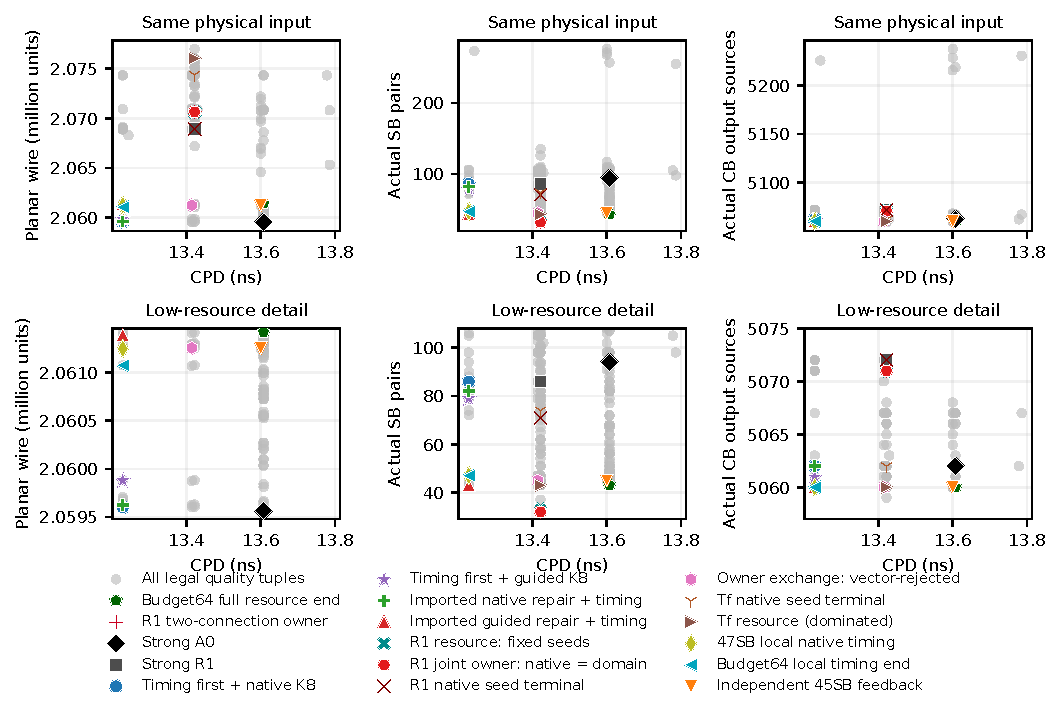
\includegraphics[width=.98\textwidth]{data/joint_quality_projection_34.pdf}
\caption{Archive 640 contains 391 BNN observations on one physical input, collapsing to 232 plotted coordinates. Both 47-SB timing menus are local terminals. Five-connection owner controls coincide; two-connection alternatives use four more wire. Budget 64 full-resource and local-timing endpoints are distinct. Inputs, roots, opportunities, full vectors and costs remain in bound data; projections are not two-dimensional Pareto boundaries.}
\label{fig:joint}
\end{figure*}

The strong native A 0 BNN root is 13.607436067 ns,2059567 wire,94 SB,5062 CB. Three current-STA strict commits reduce CPD by 2.787376\% to 13.228145690 ns for 40 wire units, keeping vertical counts. The third step regresses a noncritical setup component; strict CPD and endpoint-vector rules therefore select different trajectories. Grouped repair can also improve a setup component when its first smaller subgroup is endpoint-flat and rejected. Complete group acceptance is essential to evaluating such combinations.

Complete resource--timing pairs belong in a joint quality/cost comparison. Older imported native/domain endpoints have four/28 fewer wire than the fresh complete pair but lack comparable complete times. They remain quality observations and are not assigned the new cold costs. The archive projection retains dominated and rejected legal candidates with input identities and full vectors; coincident points are not independent samples and two-dimensional projections are not Pareto frontiers.

Fixed terminal layers require 5103 counted nonglobal networks to cross. The audited graph has unit-capacity CB sources and uniquely paired unit-capacity SB halves. Distinct networks therefore require distinct counted resources: $S+C\ge 5103$. The 43-SB/5060-CB route attains that bound; under $C\le 5060$, $S\ge 43$ is attained. This is fixed-graph vertical occupancy optimality, with no claim of optimal placement, wire or timing.

A fixed timing envelope permits other useful points. On SB-only eltwise, setting the CPD limit once to 102\% of the root allows the domain branch to reach 995 SB,227583 wire and 6.114032 ns, versus native 999 SB,227439 wire and 6.040485 ns. It trades 144 wire,1.218\% CPD and 133.56 s for four fewer SB. The envelope is development-derived, not an external application requirement or unseen-test result.

Separate BNN resource prefixes reveal a different wire/vertical tradeoff. From the same 48-SB source, a 54-connection guided group and 462-connection native group reach 47 SB; their subsequent complete local timing menus both reach 13.228145690 ns, with 2061076 versus 2061249 wire. The guided local result saves 173 wire against that local native control, but has four more SB than the complete 43-SB branch. Prefix creation, initial routing and graph preprocessing are outside those measured local timing segments. This evidence tests composition opportunity, not general complete-algorithm improvement.

Final selection is distinct from SB/CB transition acceptance. An existing Tf candidate saves 80 wire at unchanged CPD/SB/CB but changes setup components by 19 improvements/four regressions. A fixed-timing terminal rule accepts it; endpoint nonregression rejects it. The same two rules find no replacement in the two robot menus. A separately constructed BNN 2059607-wire composition remains pending its own native LOAD/FULL/STA; its structural prediction is not yet a legal measured quality point.
\section{Mechanism Ablations and Attribution}
\subsection{Domain restriction and failure release}
Domain restriction encourages cross-layer reuse under a fixed cut. Its contribution is evaluated against an unrestricted search from the same source, request, seed, scope and objective. After trajectories diverge, native and domain controls select from their own current successors. Eltwise and softmax never trigger failed-search release: their results cannot be credited to that mechanism. Softmax's equal final quality and SB-only's unfavorable strict-budget result remain negative evidence for universal domain benefit.

In an R 1 transaction, all-eight-network domain search fails at network 31767/pin 1 after five successful restorations. Under the recorded occupancy, the retained domain has no capacity path while unrestricted search has a witness. A relaxed reachability check immediately after pruning also has no domain-capacity path; later restorations only add occupancy. This establishes a fixed-scope/domain obstruction, not global unroutability.

Automatic release of only the failed network reproduces the selective-release route and full endpoint vector. It reaches 72 SB versus 74 for the matched unrestricted control, at 64 more wire and unchanged CPD/CB. Nine setup components improve with no regression; strict CPD rejects but endpoint-vector acceptance succeeds. Release preserves guidance for other networks, so its benefit must be separated from disabling all domains.

In robot's first matched transaction, a still-guided net saves one CB; two nets release their domains. A source-cut audit separates the mechanisms: every same-layer source exit is held at unit capacity by an owner outside the transaction, while the retained domain allows only outward crossing sources. A source-layer sink cannot return under that domain. Release removes this domain obstruction, but both actual candidates retain two crossings per blocked net; freeing outside owners is a separate intervention. The same-source release-only ablation remains queued, so native ablation outcomes and owner-scope gains on robot are not claimed.

\subsection{Blocking-owner coordination}
R 1's remaining excess crossing exposes a different limitation: all eight same-layer OPIN exits are owned by other nets. Fixed-scope trials preserve the extra crossing or fail with exact restoration; the 5104-resource state is a single-net local minimum. A current-margin selector adds one blocking-owner branch to the target's four connections. Unrestricted and target-CB-domain transactions both reach 2070653 wire,32 SB,5071 CB, with the original full endpoint vector unchanged. Both transfer the blocking resource and attain the 5103 terminal bound. The observed benefit is expanded coordination scope; there is no additional domain advantage in this comparison.

Reducing that intervention to two connections produces 2070657 wire with the same vertical counts and full vector in both native arms and a separately constructed BFS candidate. All are legal but dominated by the five-connection result. Two-query cores take 13.58/13.69 s against five-query 13.40/14.19 s, so fewer queries alone do not demonstrate a faster mechanism. Shared diagnostic costs are not per-arm or complete-flow measurements.

\subsection{Grouping and complete combinations}
A 64-connection budget improves one large local scope by reducing 462 queries to 54, but fails as a general trajectory optimization. Across the complete four-role budget cohort, three endpoints match K 8 quality; BNN domain ends 46 wire worse at equal CPD/SB/CB, taking 10568.53 versus 7099.32 s of imported workflow. The first four rounds have identical vectors and ordered trees. At the fifth same source, budgeting splits 77 connections into 64; both trajectories eventually execute the same 2722-query multiset, with 32 versus 18 transactions. Extra loading, STA and audits erase the local query intuition. These are descriptive development timings, not cold or statistical speedups.

Tied-path feedback supplies a complementary positive combination example. Jointly covering two tied-path targets with three donors improves ten setup components with no regression, gaining 7.638334 ps at 45 SB/5060 CB. A larger successor improves CPD further but regresses a noncritical setup component. The policy distinction is deliberate, and neither result establishes that every intermediate or module should improve CPD. Historical local trajectories and recovery costs are retained in the supplement.
\section{Overhead and Applicability}
\subsection{Engineering cost and symmetric controls}
Single-pass indexing preserves all BNN graph payloads, downstream states, requests, native work and quality at 7463.17 versus 7933.25 s. Explicit same-flow metadata plus streaming parsing also preserves that actual execution. Its original GNU-time records 7247 s (integer-second precision), versus 7463/7933 s in the same clock scope: about 216/686 s less. The observer was lost and another case briefly overlapped; complete PSS is unavailable. This qualified engineering observation neither establishes statistical acceleration nor revises the matched-pair 22.95\% domain overhead. Both arms need the same stable implementation and interleaved measurement.

Acceptance-ordered execution skips an optional native diagnostic only after the domain candidate passes full resource acceptance. On eltwise it preserves every executed candidate and selected state, reducing 64 to 32 queries and 101 to 51 attempts; whole time is 203.48 versus 289.21 s. Softmax also preserves execution with 271.70 versus 336.68 s. With no eligible cut, SPMV skips no work and takes 93.15 versus 91.55 s. Unexecuted diagnostics have no imputed metrics.

Combining lazy scheduling with in-call source snapshots preserves the actual states, requests, skipped roles and work. Eltwise takes 198.88 s versus 203.48 s, softmax 256.54 s versus 271.70 s. Conversely, fused FULL/STA alone preserves quality but costs 313.74 versus 289.21 s on eltwise. Engineering changes therefore need complete measured controls; reducing processes or a nested core does not establish end-to-end benefit.

Every elapsed time belongs to one declared command and output. Cold graph construction and explicitly supplied reusable indexes are different cost modes. Shared-machine concurrency and OS caches are uncontrolled. After version stability, the matched arms require same-environment interleaved repetitions, including failures, rather than selecting the fastest observation. Recovery segments, component cores and one-time research validation are reported separately and never summed into a fabricated complete time.

\subsection{Evidence coverage and confirmation boundary}
The 671-record archive includes 34 quality-complete modern configurations on five known successful circuits and three vertical families, not independent samples. Of these, 33 have complete observer measurements; the streaming control has qualified GNU-time only. Its 13 actual states include legal rejected candidates; only its final state carries the elapsed time. Initial failures remain outside legal-quality counts and inside cohort denominators.

Applicable graphs here are two-layer edge-encoded Hybrid-O, SB-only and CB-only. Flat routing, CHANZ, general multilayer devices, altered placements and broad timing-constrained application suites remain unconfirmed. CB-only's 982 crossing nets saturate the 982-source terminal lower bound; this says nothing about wire or CPD optimality. No-cut, equal-quality, worse-quality and initial-failure inputs remain part of the scope statement.

The next confirmation artifact must be independently executable with fixed source/binary hashes, mechanism triggers, candidate order, acceptance envelope and terminal policy. Its native arm receives matching group selection, scope expansion and convergence opportunities. Domain, release and owner switches are separately varied on the same inputs for attribution. Development threshold exploration must not silently modify that artifact or reuse confirmation outcomes to select a new rule within the same cohort.

Independent input identity binds netlist, architecture, actual placement coordinates, constraints and initial route trees. Different seed labels with identical trees do not count as different starts; distinct routing starts on one placement and distinct placements are reported separately. Candidate inputs are selected before policy outcomes, and every registered failure is retained. Since BNN currently uses default constraints, application timing claims additionally require new paired instances with explicit SDC clocks and I/O requirements~\cite{vprsdc}; a development-relative CPD cap is not such a requirement.

The supported claims are therefore specific: complete BNN resource/time tradeoffs, positive and negative circuit/topology transfer, and matched local mechanism effects. Broad superiority of the fully integrated controller, timing-closure guarantees, silicon-area savings and statistical acceleration are not established.
\begin{thebibliography}{4}
\bibitem{vtr9paper} M. A. Elgammal et al., ``VTR 9: Open-source CAD for fabric and beyond FPGA architecture exploration,'' \emph{ACM Trans. Reconfigurable Technol. Syst.}, 2025, doi:10.1145/3734798.
\bibitem{flatland} C. Hao, A. B. Kahng, B. Pramanik, and I. Youssef, ``Escaping Flatland: A placement flow for enabling 3D FPGAs,'' in \emph{Proc. ACM/IEEE DAC}, 2026, doi:10.1145/3770743.3804424.
\bibitem{pathfinder} L. McMurchie and C. Ebeling, ``PathFinder: A negotiation-based performance-driven router for FPGAs,'' in \emph{Proc. FPGA}, 1995, pp.111--117.
\bibitem{vprsdc} Verilog-to-Routing, ``Timing constraints,'' \url{https://docs.verilogtorouting.org/en/latest/vpr/timing_constraints/}, accessed Nov.15,2026.
\end{thebibliography}
\end{document}
